\chapter{The World of \ourgame{}}
\section{Setting}
\ourgame{} is set primarily in the modern age, in a world very much like the player's own. The main environment is Omar Clean's mansion. From the outside, the mansion is a decently large Palladian-inspired building, similar to Figure~\ref{fig:mansion_photo}. On the inside, the rooms are modestly sized, conservatively designed, and unassuming. However, as one explores the rooms of the mansion, it becomes clear that it is larger on the inside than the outside. Much, much larger. Impossibly large. And doors start to lead to impossible places, like giant forests, or dockside crime lairs.

\begin{figure}[htb]
\centering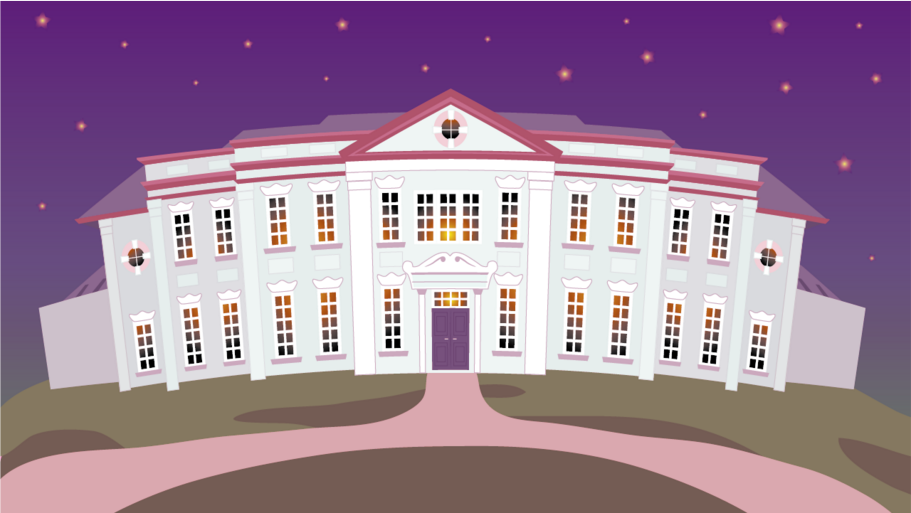
\includegraphics[width=.4\linewidth]{images/mansion2}
\caption{Concept artwork of Omar's mansion, inspired by neo-Palladian English architecture.}
\label{fig:mansion_photo}
\end{figure}

The game environment is rendered in 3D using a stylized cartoon aesthetic. It is populated by many unique characters. Most appear to be human but it is clear that the inhabitants of this world are more than they seem. They can have brightly-coloured skin, outrageous body types, and even animal parts. The characters are rendered in the game environment as 2D billboards to create an off-kilter visual style, similar to those in Figure~\ref{fig:render_style}.

\begin{figure}[htb]
  \centering%
  \begin{subfigure}{.33\textwidth}
    \centering
    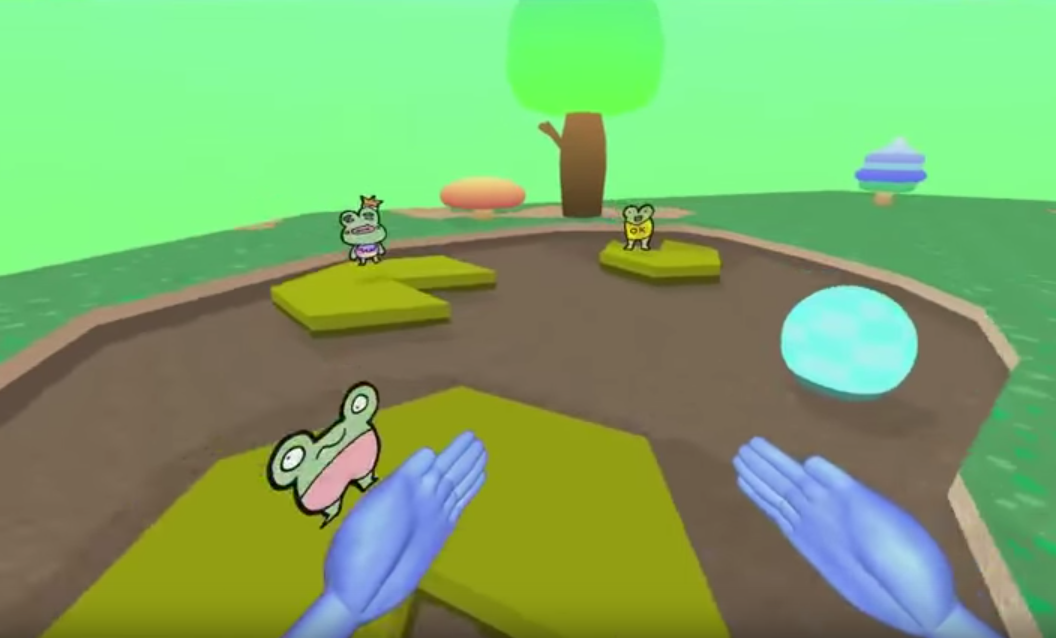
\includegraphics[width=.9\linewidth]{images/burrito}
  \end{subfigure}%
  \begin{subfigure}{.33\textwidth}
    \centering
    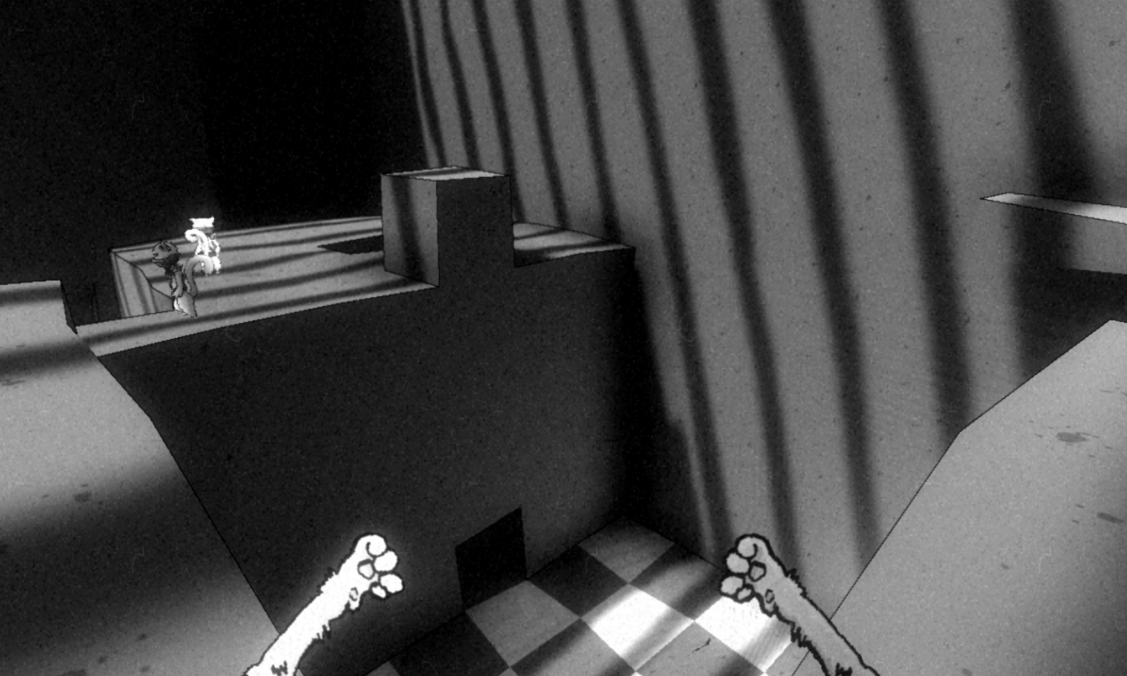
\includegraphics[width=.9\linewidth]{images/sketchtales}
  \end{subfigure}%
  \caption{The upcoming games \textit{Burrito Galaxy 65} and \textit{Sketch Tales} both render 2D characters in stylized and cartoon 3D worlds.}
  \label{fig:render_style}
\end{figure}

Throughout the game, the player can travel to alternate dimensions. Every playthrough occurs within Omar Clean's mansion, but the mansion changes in subtle ways. The style and interior design remain the same, but the floor layout, furniture, items, and character designs all change and shift between dimensions. The mansion is always owned by Omar Clean, but each dimension has its own unique version of Omar -- sometimes an adventurer, sometimes a scientist, sometimes a robot. 

The protagonist of \ourgame{} is a blank slate. The player controls this character, and can project their own impressions and assumptions with them into the world, which shapes the way they interpret their surroundings, and their purpose within \ourgame{}.
\section{Main Plot}
\label{sec:mainplot}
The game begins at the player's desk. Ballpoint pens and other trinkets cover the surface. In the centre of the desk lies an envelope with an elaborate wax seal. The player opens the letter and finds an invitation to a party, courtesy of one Omar Clean. The player arrives at the party and hands their invitation to the mansion's kindly old butler, who leads them through the anteroom into the main part of the house. There, the player is greeted by the party's host, the mysterious Omar Clean. Omar is almost immediately bludgeoned to death by an unknown assailant, who then knocks the player unconscious.

The player awakes to find a private investigator named Goodsee Beauregard. Beauregard interrogates the player about the murder, and explains that she has spent several weeks investigating Omar Clean for suspicious behaviour. She asks the player to help her track down Omar's killer and find some answers. The player's quest to unlock the mysteries of the house begins.

The player starts by searching the house for the murderer, asking other party-goers for any information they have to spare and finding clues. Their investigation leads them to a secret room, where they finds the murderer standing in front of a giant electronic machine. A bright flash blinds the player. After regaining their sight, they find themselves once again outside of the house.

The player re-enters the mansion and retraces their steps from their first arrival. The butler's behaviour and the anteroom are all identical. Once the player enters the mansion, however, they find the layout of the house, its furniture, and the party-goers to be different. The player meets Omar Clean, very much alive, and very much a different person than the murder victim. The player discovers that the mysterious machine transported them to an alternate dimension. They proceed to travel between dimensions to solve the mystery of Omar Clean, and to find a way back home.

The player progresses through multiple dimensions by discovering clues and tracking down different versions of Omar Clean, whom the player can use as portals. After travelling through several of these self-contained dimensions, they stumble upon a house that is different from all the others. There is no party. The house looks decrepit and unkempt, and there are no guests at all. Amid the wreckage, the player finds the machine from before. Above it sits a giant portrait of a man who looks like he has been dead for many years. A voice comes from within the painting and introduces itself as Omar Clean. He tells the player how he was trapped in the painting by the Omars of other dimensions, forced to take on their weaknesses as they live their lives free of pain and death. The murderer appears and confronts the player, revealing himself to be another version of Omar Clean. He tells the player that the painting is lying -- the Omar in the painting tried to steal the life-force from all the other Omars, but ended up absorbing their weakness. He sealed himself inside the painting to preserve his body in the hopes that someone would rescue him and allow him to re-enact his plan. The "murderer" Omar explains that he travels between dimensions to protect the painting from harm. If the painting is destroyed, the weaknesses within are returned to their respective Omars, who will all die from the strain.

The player can decide to trust the Painting Omar, trust the Protector Omar, or destroy the painting. If they choose to side with Painting Omar, he regains his human form and kills the other Omar. He tells the player he will kill the other Omars and rule over all dimensions. Painting Omar activates the interdimensional transportation device, and the player sees a bright flash of white light. The game ends.

If the player trusts the Protector Omar, he thanks the player and activates the interdimensional transportation device, taking the player back to their own dimension. The party there continues on into the night as if nothing happened at all.

If the player destroys the painting, Painting Omar dies. Protector Omar curses at the player as his body splits apart and collapses to the ground. The player can then activate the machine and return to their dimension, where the party is somehow still going on. People dance, Goodsee searches for Omar, and everything seems to be the same as when the player started. The guests still whisper to each other about the reclusive Omar Clean, wondering if they will ever get a chance to meet him in person.
\section{Side Plots}
Most of the alternate dimensions within \ourgame{} have a particular version of Omar Clean. Each version of Omar Clean has their own desires and issues within their own dimension. The player can choose to help or hinder each Omar in their personal quests. These quests do not change the outcome of the main plot, but serve to endear the player to the multiple Omar Cleans, and to give them a secondary motivation for exploring the many dimensions in the game world. Examples of these secondary Omar Cleans can be found in Appendix \ref{app:characters}.

Each run will also include characters who will ask the player to solve certain problems for them in exchanges for items or access to new parts of the mansion. These stories will be small and self-contained. Examples of these secondary plots and the characters involved can be found in Appendix \ref{app:characters}.


\clearpage
\section{Characters}

\subsection{Main Characters}
Main characters are characters directly related to the main storyline described in Section~\ref{sec:mainplot}. This includes Goodsee Beauregard, the Protector version of Omar Clean, and the Portrait version of Omar Clean, who are described in more detail in Appendix \ref{app:characters}.

\subsection{Side Characters}
Side characters are characters that are not involved with the main storyline, but are involved in secondary storylines in \ourgame{}. These storylines are small and contained, and they resolve with help from the player. Upon completing these smaller stories, the player gets rewards that may aid them in completing the main storyline. Examples of side characters can be found in Appendix~\ref{app:characters}.

\subsection{Incidental Characters}
Many characters in \ourgame{} are simple party guests with no relation to the main storyline or any side plots. These characters will be procedurally generated using a component structure. Lines of semi-procedurally generated dialogue will be created for each character that will be said when the player interacts with the character. This use of procedural generation allows for the reuse of assets to quickly and uniquely populate each environment with interactive characters, without feeling overly repetitive for the player.